\chapter{Capability Stacking in Real Estate}

A real estate license can be treated as a narrow job ticket, or it can be treated as the beginning of a broader commercial skill set. The speaker begins with the ordinary post-license path, names the way brokerage training often narrows a person into one role, and then pivots to TRE's preferred word: entrepreneur. We will use a small amount of notation to make the mechanism precise, but the source claim remains practical: when the market shifts, a one-lane operator has fewer ways to respond.

\paragraph{Source note.} This chapter is based on a School of Hard Knocks entrepreneurship interview, curated by LazyingArt LLC through Video2Book.

\section{A License Followed By A Narrowing}

We begin where the speaker begins: in the real estate brokerage world, after the license. The license is the entry point. The narrowing comes afterward, when the new agent is typically taught to ``just do one thing.'' That phrase is the first important object in the argument. It is not only a training recommendation; it is a constraint on what the new professional learns to see.

The transcript then moves through examples in a deliberately repetitive way. A person may be taught to be a listing agent, to do residential, to be a buyer's agent, to do only commercial, not to do residential, not to worry about investing, and not to wholesale. We can collect the named lanes as
\begin{equation}
\mathcal{R}
=
\{
\text{listing},
\text{residential},
\text{buyer-side},
\text{commercial},
\text{investing},
\text{wholesaling}
\}.
\end{equation}
The set notation is editorial bookkeeping. Its purpose is to preserve the speaker's list without flattening it into a generic statement about diversification.

A narrow training path selects one lane and lets the other lanes fade from the agent's working map. In notation,
\begin{equation}
C_{\text{single}}=\{c\},
\qquad
c\in \mathcal{R},
\end{equation}
where \(C_{\text{single}}\) denotes the capability set of a professional trained into one main activity. The point is not that specialization is always wrong. The point is that specialization can become a hidden ceiling when the person is not equipped to move when the market moves.

\section{Naming The Wider Operator}

The pivot comes when the speaker says that TRE calls everybody there entrepreneurs. The word is not being used as a decoration. It renames the professional from a person attached to one brokerage lane into a person expected to operate across the real estate field.

\begin{definition}
A capability set \(C\) is the set of real estate activities a professional can actually use to create or respond to income opportunities. A single-lane agent has a small capability set. An entrepreneur, in the speaker's sense, is trained toward a wider capability set across multiple real estate lanes.
\end{definition}

The contrast is therefore
\begin{equation}
C_{\text{single}}
\subset
C_{\text{stack}},
\end{equation}
where \(C_{\text{stack}}\) is the broader capability stack TRE wants its people to build. This inclusion should be read modestly. It does not say that every professional must do every activity at once. It says that the wider operator has more available moves than the one-lane operator.

\subsection{Question \& Answer}

\paragraph{Question.} If real estate brokerage already has recognizable specialties, why not simply master one of them?

\paragraph{Answer.} The speaker's answer is the market shift. If the market changes and we do not know how to do this or that, then we are limited in how much money we can make and how successful we can be. The issue is not a slogan about being well-rounded. It is exposure to a changing environment.

The causal skeleton is
\begin{equation}
\text{market shift}
+
\text{single-lane capability}
\Longrightarrow
\text{limited earning capacity}.
\end{equation}
This is the local tension and resolution of the segment. A lane may be profitable while the market rewards that lane. The obstacle appears when the market asks for a different move.

\section{Market Shifts And The Option Model}

Let \(m\) denote the current market condition, and let \(C\) denote the practitioner's capability set. Then the income opportunity available to that practitioner can be represented abstractly as
\begin{equation}
I=I(m,C).
\end{equation}
This is not an empirical income formula. It is a disciplined way to state the transcript's mechanism: opportunity depends both on the market and on what the professional knows how to do.

To make the point concrete, suppose each capability \(c\) has an opportunity value \(i(m,c)\) under market condition \(m\). If the professional can choose among the capabilities they possess, a simple option model is
\begin{equation}
I(m,C)=\max_{c\in C} i(m,c).
\end{equation}
The maximum is not meant to predict a paycheck. It expresses a more basic fact: if additional capabilities are genuinely available options, then a larger option set cannot reduce the best available move.

\begin{proposition}
Assume \(C_{\text{single}}\subset C_{\text{stack}}\), and assume additional capabilities are options rather than obligations. Then, for any market condition \(m\),
\begin{equation}
I(m,C_{\text{stack}})
\geq
I(m,C_{\text{single}}).
\end{equation}
\end{proposition}

\begin{proof}
Using the option model,
\begin{align}
I(m,C_{\text{single}})
&=
\max_{c\in C_{\text{single}}} i(m,c),\\
I(m,C_{\text{stack}})
&=
\max_{c\in C_{\text{stack}}} i(m,c).
\end{align}
Since \(C_{\text{single}}\subset C_{\text{stack}}\), every capability available to the single-lane professional is also available inside the stacked set. Taking a maximum over the larger set cannot give a smaller result:
\begin{equation}
\max_{c\in C_{\text{stack}}} i(m,c)
\geq
\max_{c\in C_{\text{single}}} i(m,c).
\end{equation}
Therefore \(I(m,C_{\text{stack}})\geq I(m,C_{\text{single}})\).
\end{proof}

\begin{remark}
The model intentionally leaves out training cost, execution quality, distraction, and risk. Those are real business concerns, but they are not the mechanism stated in this excerpt. The speaker's narrower claim is that market shifts punish professionals who only know one lane.
\end{remark}

\section{The Mechanism In One Flow}

The spoken argument forms a compact sequence: license, narrow training, single lane, market shift, income limit, and then the alternative of entrepreneurial capability stacking. The following figure is a reconstruction of that sequence.

\begin{figure}
\centering
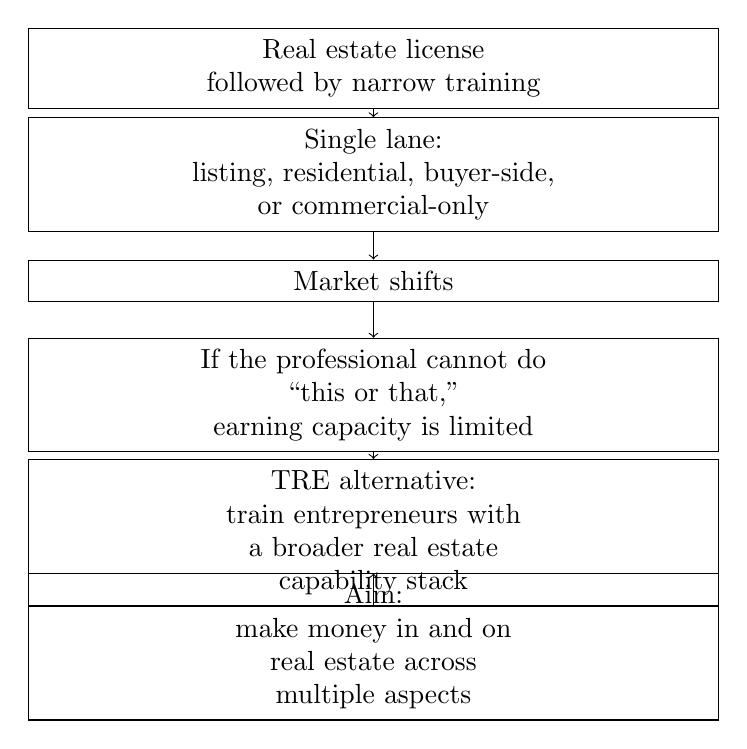
\begin{tikzpicture}[x=1cm,y=1cm]
\node[draw, align=center, text width=0.70\linewidth, inner sep=4pt] (a) at (0,0)
{Real estate license\\followed by narrow training};
\node[draw, align=center, text width=0.70\linewidth, inner sep=4pt] (b) at (0,-1.35)
{Single lane:\\listing, residential, buyer-side,\\or commercial-only};
\node[draw, align=center, text width=0.70\linewidth, inner sep=4pt] (c) at (0,-2.70)
{Market shifts};
\node[draw, align=center, text width=0.70\linewidth, inner sep=4pt] (d) at (0,-4.15)
{If the professional cannot do\\``this or that,''\\earning capacity is limited};
\node[draw, align=center, text width=0.70\linewidth, inner sep=4pt] (e) at (0,-5.90)
{TRE alternative:\\train entrepreneurs with\\a broader real estate\\capability stack};
\node[draw, align=center, text width=0.70\linewidth, inner sep=4pt] (f) at (0,-7.35)
{Aim:\\make money in and on\\real estate across\\multiple aspects};

\draw[->] (a) -- (b);
\draw[->] (b) -- (c);
\draw[->] (c) -- (d);
\draw[->] (d) -- (e);
\draw[->] (e) -- (f);
\end{tikzpicture}
\caption{A reconstruction of the speaker's sequence: narrow training creates exposure to market shifts; capability stacking is presented as TRE's alternative.}
\end{figure}

The vertical order is important. We do not begin with an abstract doctrine of entrepreneurship. We begin with the license, then the narrowing of professional identity, then the pressure of a shifting market. Only after that does the broader entrepreneurial model become necessary.

\section{Making Money In And On Real Estate}

The segment closes with the phrase that TRE teaches entrepreneurs how to make money ``in and on'' real estate, and how to make money in every aspect of real estate. We should preserve that phrase because it is the speaker's own summary of the operating model.

A cautious reconstruction is
\begin{equation}
C_{\text{stack}}
\approx
C_{\mathrm{in}}\cup C_{\mathrm{on}},
\end{equation}
where \(C_{\mathrm{in}}\) refers to capabilities inside brokerage activity and \(C_{\mathrm{on}}\) refers to adjacent real estate activity, such as investing or wholesaling. The approximation sign matters. The transcript does not define a clean taxonomy of ``in'' and ``on,'' so the notation should remain a guide, not a doctrine.

Read in ordinary business language, the claim is that real estate is not one job. It is a field with several ways to create value: representation, listing, buyer-side work, residential activity, commercial activity, investing, wholesaling, and other adjacent moves. The one-lane professional is exposed to the fortunes of one channel. The entrepreneur is trained to notice more channels and to move when the market changes.

\section{Summary}

The argument unfolds in a short but coherent sequence. First, the speaker places us in the brokerage world after licensing. Then he names the common narrowing: the new professional is taught to do one thing. He gives the narrowing concrete form by listing the lanes that are often separated from one another. TRE's pivot is to call its people entrepreneurs, meaning real estate professionals whose capabilities extend beyond one assigned role.

The working model is
\begin{equation}
I=I(m,C):
\end{equation}
income opportunity depends on both the market condition \(m\) and the capability set \(C\). The transcript gives no commission rates, probabilities, income figures, or formal investment model, so the mathematics must stay modest. Its durable lesson is that a market shift can turn a single capability into a ceiling, while a broader capability stack gives the entrepreneur more possible moves in and on real estate.